% =========================================================================== %

\begin{frame}[t,plain]
\titlepage
\end{frame}

% =========================================================================== %

\begin{frame}{Recap}
%
\begin{columns}[T]
\column{.5\linewidth}
\begin{itemize}
\item \inPy{while}-Schleifen
	\begin{itemize}
	\item Wiederholung, solange eine Bedingung erfüllt ist
	\end{itemize}
\item \inPy{break} und \inPy{continue} bei Schleifen
	\begin{itemize}
	\item Schleife vorzeitig verlassen (\inPy{break}) bzw. vorzeitig neu beginnen (\inPy{continue})
	\end{itemize}
\item \inPy{else} bei \inPy{for} und \inPy{while}
	\begin{itemize}
	\item \inPy{for}  -- Ausführung bei Erreichen des Schleifen-Endes
	\item \inPy{while} -- Ausführung, wenn Schleifenkörper nie betreten wird
	\end{itemize}
\end{itemize}
%
\column{.5\linewidth}
\begin{itemize}
\item Funktionen
	\begin{itemize}
	\item Abgetrennte Code-Abschnitte für wiederkehrende Aufgaben
	\item Variablen nicht überall sichtbar (\thus Scopes)
	\item Änderungen nur bei \emph{mutable} Variablen
	\item Speicherbild -- alte Referenzen mit neuen (lokalen) Namen
	\end{itemize}
\end{itemize}

\end{columns}
%
\begin{center}
	\emph{Noch Fragen?}
\end{center}
%
\end{frame}

% =========================================================================== %

\begin{frame}[fragile]{Kapitel 6}
%
\begin{itemize}
\item Optionale Parameter
\item Variadische Funktionen
\item Funktionen als Rückgabewerte
\item Lambdas
\item Rekursion
\end{itemize}
%
\end{frame}

% =========================================================================== %

\begin{frame}[fragile]{Optionale Parameter}
%
\begin{columns}[T]
\column{.5\linewidth}
\begin{itemize}
\item Recap: Funktionen erlauben kompakte Lösung wiederkehrender Aufgaben
\item Parametrisierbar -- Liste von Werten, die für die Funktion verwendet werden
\item Häufig: Standardwerte, die jedes Mal wieder gebraucht werden
\item Spezielle Syntax: Standardwerte bei Aufruf dann optional
\end{itemize}
%
\column{.5\linewidth}
\begin{codebox}[Syntax: Optionale Parameter]
\begin{minted}[fontsize=\scriptsize]{python}
def Funkname (param, optParam = Wert) :
    ...
\end{minted}
\end{codebox}
%
\begin{codebox}[Syntax: Aufruf mit opt. Parametern]
\begin{minted}[fontsize=\scriptsize]{python}
Funkname (param)
Funkname (param, optParam)
\end{minted}
\end{codebox}
\end{columns}
%
\end{frame}

% =========================================================================== %

\begin{frame}[fragile]{Optionale Parameter}
%
\begin{columns}[T]
\column{.5\linewidth}
\begin{itemize}
\item Beliebig viele \emph{positionale} (normale) Parameter
\item Beliebig viele optionale Parameter
\item Optionale Parameter immer am Ende
\item Beim Aufruf: nur von hinten herein auslassbar
\end{itemize}
%
\column{.5\linewidth}
\begin{codebox}[Beispiel: Aufruf mit opt. Parametern]
\begin{minted}[linenos, fontsize=\scriptsize]{python}
# def func (a, b = 2, c) :
#    letzter Parameter nicht opt.

def func (a, b = 2, c = 3) :
    print(a, b, c)
    
func(1)
func(-1, -2)
func(-1, -2, -3)
# func(-1, , -3) ausgelassener Parameter
\end{minted}
\end{codebox}
\end{columns}
%
\end{frame}

% =========================================================================== %

\begin{frame}[fragile]{Variadische Funktionen}
%
\begin{columns}[T]
\column{.5\linewidth}
\begin{itemize}
\item Manche Funktionen erlauben beliebige Anzahl von Parametern
\item Vgl. \inPy{print}
\item Umgesetzt durch eigene Syntax
\item Übergabe als \inPy{tuple}
\end{itemize}
%
\column{.5\linewidth}
\begin{codebox}[Syntax: Variadische Funktionen]
\begin{minted}[fontsize=\scriptsize]{python}
def Funkname (params, *varArg) :
    ...
\end{minted}
\end{codebox}
%
\begin{codebox}[Syntax: Aufruf Variadische Fktn.]
\begin{minted}[fontsize=\scriptsize]{python}
Funkname (param)
Funkname (param, varArg1, varArg2, ...)
\end{minted}
\end{codebox}
\end{columns}
%
\end{frame}

% =========================================================================== %

\begin{frame}{Variadische Funktionen}
%
\begin{itemize}
\item Beliebig viele feste Parameter vor den variadischen
\item Maximal ein variadischer Parameter -- nimmt alle übrigen auf
\item Beliebig viele optionale Parameter \emph{vor oder nach} dem Variadischen
	\begin{itemize}
	\item Zuordnung dann beim Aufruf durch Klausel \inPy{optParam = Wert}
	\item Siehe später mehr hierzu
	\end{itemize}
\end{itemize}
%
\end{frame}

% =========================================================================== %

\begin{frame}[fragile]
%
\begin{tcbraster}[raster columns=2,
                  raster equal height,
                  nobeforeafter,
                  raster column skip=0.5cm]
\begin{codebox}[Beispiel: Variadische Funktionen]
\begin{minted}[linenos, fontsize=\scriptsize]{python}
def func (
    posArg1, posArg2,
    *varArg,
    optArg = 0
) :
    print("pos. arguments:",
          posArg1, posArg2)
    print("var. argument :", varArg)
    print("opt. argument :", optArg)
    print()

func(1, 2)
func(1, 2, 3, 4, 5, 6, "sieben")
func(1, 2, 3, optArg = 4)
func(1, 2, optArg = 3)
\end{minted}
\end{codebox}
%
\begin{cmdbox}[Ausgabe: Variadische Funktionen]
\begin{minted}[fontsize=\scriptsize]{text}
pos. arguments: 1 2
var. argument : ()
opt. argument : 0

pos. arguments: 1 2
var. argument : (3, 4, 5, 6, 'sieben')
opt. argument : 0

pos. arguments: 1 2
var. argument : (3,)
opt. argument : 4

pos. arguments: 1 2
var. argument : ()
opt. argument : 3
\end{minted}
\end{cmdbox}
\end{tcbraster}
%
\end{frame}

% =========================================================================== %

\begin{frame}[fragile]{Schlüsselwort-Parameter}
%
\begin{columns}[T]
\column{.5\linewidth}
\begin{itemize}
\item Wie variadische Parameter: Übergabe von Schlüssel-Wert-Paaren
\item Umgesetzt durch eingene Syntax
\item Übergabe als \inPy{dict}
\item Bei Aufruf: Paare von \inPy{Schlüssel = Wert}
\end{itemize}
%
\column{.5\linewidth}
\begin{codebox}[Syntax: Variadische Funktionen]
\begin{minted}[fontsize=\scriptsize]{python}
def Funkname (params, **kwargs) :
    ...
\end{minted}
\end{codebox}
%
\begin{codebox}[Syntax: Aufruf Variadische Fktn.]
\begin{minted}[fontsize=\scriptsize]{python}
Funkname (par)
Funkname (par, kw1 = v1, kw2 = v2, ...)
\end{minted}
\end{codebox}
\end{columns}
%
\end{frame}

% =========================================================================== %

\begin{frame}{Schlüsselwort-Parameter}
%
\begin{itemize}
\item Beliebig viele Schlüsselwort-Parameter
\item Reihenfolge:
	\begin{itemize}
	\item positionale Parameter
	\item optionale Parameter
	\item variadische Parameter
	\item Schlüsselwort-Parameter
	\end{itemize}
\end{itemize}
%
\begin{hintbox}[Gedankenstütze für Reihenfolge]
Der Interpreter muss bei jedem Aufruf entscheiden können, welche Werte zu welchen Parametern gehören. Dies ist nur bei der genannten Anordnung möglich.
\end{hintbox}
%
\end{frame}

% =========================================================================== %

\begin{frame}[fragile]
%
\begin{tcbraster}[raster columns=2,
                  raster equal height,
                  nobeforeafter,
                  raster column skip=0.5cm]
\begin{codebox}[Beispiel: Variadische Funktionen]
\begin{minted}[linenos, fontsize=\scriptsize]{python}
def func (
    posArg1, posArg2,
    optArg = 0,
    *varArg, **kwArg
) :
    print("pos. arguments:",
          posArg1, posArg2)
    print("var. argument   :", varArg)
    print("opt. argument   :", optArg)
    print("key. argument   :", kwArg)
    print()

func(1, 2, 3)
func(1, 2, key="value")
func(1, 2, optArg="value")
# func(1, 2, 3, optArg="value")
# doppelter Wert für optArg!
func(1, 2, "value", 4, key="value")
\end{minted}
\end{codebox}
%
\begin{cmdbox}[Ausgabe: Variadische Funktionen]
\begin{minted}[fontsize=\scriptsize]{text}
pos. arguments: 1 2
var. argument   : ()
opt. argument   : 3
key. argument   : {}

pos. arguments: 1 2
var. argument   : ()
opt. argument   : 0
key. argument   : {'key': 'value'}

pos. arguments: 1 2
var. argument   : ()
opt. argument   : value
key. argument   : {}

pos. arguments: 1 2
var. argument   : (4,)
opt. argument   : value
key. argument   : {'key': 'value'}
\end{minted}
\end{cmdbox}
\end{tcbraster}
%
\end{frame}

% =========================================================================== %

\begin{frame}[fragile]{Optionale Parameter bei \inPy{print}}
%
\begin{columns}[T]
\column{.5\linewidth}
\begin{itemize}
\item \texttt{end} -- Zeichen(kette), die automatisch \emph{nach dem letzten Parameter} gedruckt wird. Standardmäßig \inPy{"\n"} (Zeilenumbruch)
\item \texttt{sep} -- Zeichen(kette), die automatisch \emph{zwischen zwei} Parametern gedruckt wird. Standardmäßig \inPy{" "} (Leerzeichen)
\item \texttt{file} -- Ziel\enquote{datei}, in die geschrieben wird (Standardmäßig der \enquote{Bildschirm})
\item \texttt{flush} -- automatisches aktualisieren (standardmäßig \inPy{False})
\item Signatur \inPy{def print(*values, sep=' ', end='\n', file=sys.stdout, flush=False)}
\end{itemize}
%
\column{.5\linewidth}
\begin{codebox}[Beispiel: Opt. Params bei \texttt{print}]
\begin{minted}[linenos, fontsize=\scriptsize]{python}
print(1, 2, 3)
print(1, 2, 3, sep="--")
print(1, 2, 3, end="#\n")
print(1, 2, 3, end="#\n", sep="--")
\end{minted}
\end{codebox}
%
\begin{cmdbox}[Ausgabe: Variadische Funktionen]
\begin{minted}[fontsize=\scriptsize]{text}
1 2 3
1--2--3
1 2 3#
1--2--3#
\end{minted}
\end{cmdbox}
\end{columns}
%
\end{frame}

% =========================================================================== %

\begin{frame}[fragile]{Funktionen als Rückgabewerte}
%
\begin{itemize}
\item In Python kann \emph{alles} in Variablen gespeichert werden
\item[\Thus] alles kann auch Rückgabewert einer Funktion sein
\end{itemize}
%
\begin{tcbraster}[raster columns=2,
                  raster equal height,
                  nobeforeafter,
                  raster column skip=0.5cm]
\begin{codebox}[Beispiel: Funktionen zurückgeben]
\begin{minted}[linenos, fontsize=\scriptsize]{python}
import math

def funcSelector (funcNummer) :
    if funcNummer == 1 :
        return math.sin
    elif funcNummer == 2 :
        return math.cos

func = funcSelector(2)
print(func)
print(func(math.pi))
\end{minted}
\end{codebox}
%
\begin{cmdbox}[Ausgabe: Variadische Funktionen]
\begin{minted}[fontsize=\scriptsize]{text}
<built-in function cos>
-1.0
\end{minted}
\end{cmdbox}
\end{tcbraster}
%
\end{frame}


% =========================================================================== %

\begin{frame}[fragile]
%
\begin{hintbox}[Lookups über \texttt{dict}s]
\scriptsize
Das vorige Beispiel soll nur die Idee illustrieren. Lange \inPy{if-elif-...}-Ketten lassen sich durch \inPy{dict}s ersetzen:

\begin{codebox}[Beispiel: Lookups mit \texttt{dict}s]
\begin{minted}[linenos, fontsize=\scriptsize]{python}
import math
funcSelector = {1 : math.sin,
                2 : math.cos}
func = funcSelector[1]
print(func, func(math.pi))
\end{minted}
\end{codebox}
\end{hintbox}
%
\begin{hintbox}[Syntax-Element Klammern]
Ohne Klammern -- \emph{Nennung} des Objekts (Funktion)\\
Mit Klammern -- \emph{Aufruf} des Objekts
\end{hintbox}
%
\end{frame}

% =========================================================================== %

\begin{frame}[fragile]{Funktionsgeneratoren}
%
\begin{itemize}
\item Funktionen können ineinander geschachtelt werden
\item Die innere Funktion kann zurück gegebeben werden
\item Die innere Funktion wird für jeden Aufruf der äußeren neu angelegt
\item Parameter werden jeweils in das neu generierte Objekt eingesetzt
\item Erlaubt also \emph{dynamisches Erzeugen} von Funktionen
\end{itemize}
%
\end{frame}

% =========================================================================== %

\begin{frame}[fragile]
%
\begin{tcolorbox}[title=Differentialquotient]
	\begin{equation*}
	\dv{x} f(x)
=
	\lim_{\varepsilon \to 0}
		\frac
			{f(x + \varepsilon) - f(x)}
			{\varepsilon}
	\end{equation*}
\end{tcolorbox}
%
\begin{codebox}[Beispiel: Numerisches Ableiten]
\begin{minted}[linenos, fontsize=\scriptsize]{python}
import math

def derivative (f, epsilon = 1e-7) :
    def result(x) :
        return (f(x + epsilon) - f(x)) / epsilon
    return result

dsin = derivative(math.sin)
dcos = derivative(math.cos)

for x in range(20) :
    print(int(20 + 10 * dsin(x / 3)) * " ", "*")
\end{minted}
\end{codebox}
%
\end{frame}

% =========================================================================== %

\begin{frame}[fragile]
%
\begin{codebox}[Beispiel: Funk.gen, width=.333\linewidth, nobeforeafter, equal height group=A]
\begin{minted}[fontsize=\scriptsize, linenos, firstnumber=last]{python}
print(derivative)
print(dsin)
print(dcos)
\end{minted}
\end{codebox}
%
\begin{cmdbox}[Ausgabe: Funktionsgeneratoren, width=.655\linewidth, nobeforeafter, equal height group=A]
\begin{minted}[fontsize=\scriptsize]{text}
<function derivative at 0x7f44162a7940>
<function derivative.<locals>.result at 0x7f44264a9820>
<function derivative.<locals>.result at 0x7f44243b21f0>
\end{minted}
\end{cmdbox}
%
\begin{tcolorbox}[title=Speicherbild]
\begin{center}
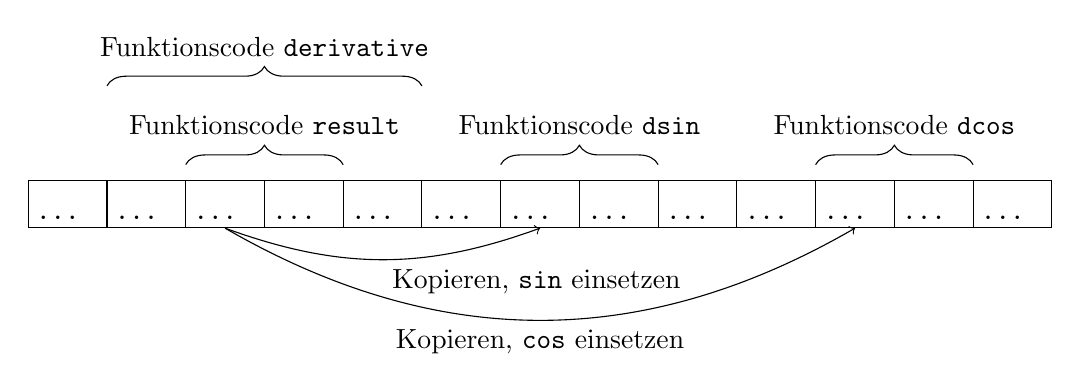
\begin{tikzpicture}
  [ 
    cell/.style={text width=8mm,
      text height=4mm, draw=black, inner sep=1mm},
    ld/.style={draw=blue,shorten >=2pt,->}
  ]
  \node  (a0) at ( 0,0) [cell] {\ttfamily ...};
  \node  (a1) at ( 1,0) [cell] {\ttfamily ...};
  \node  (a2) at ( 2,0) [cell] {\ttfamily ...};
  \node  (a3) at ( 3,0) [cell] {\ttfamily ...};
  \node  (a4) at ( 4,0) [cell] {\ttfamily ...};
  \node  (a5) at ( 5,0) [cell] {\ttfamily ...};
  \node  (a6) at ( 6,0) [cell] {\ttfamily ...};
  \node  (a7) at ( 7,0) [cell] {\ttfamily ...};
  \node  (a8) at ( 8,0) [cell] {\ttfamily ...};
  \node  (a9) at ( 9,0) [cell] {\ttfamily ...};
  \node (a10) at (10,0) [cell] {\ttfamily ...};
  \node (a11) at (11,0) [cell] {\ttfamily ...};
  \node (a12) at (12,0) [cell] {\ttfamily ...};
  
  \draw [decorate, decoration={brace,amplitude=7pt}, xshift=-0pt, yshift=0pt]
  		( 0.5, 1.5) -- ( 4.5, 1.5) node [midway, yshift=+0.5cm] 
		(braceFuncDerivative) {Funktionscode \texttt{derivative}};
	
  \draw [decorate, decoration={brace,amplitude=7pt}, xshift=-0pt, yshift=0pt]
  		( 1.5, 0.5) -- ( 3.5, 0.5) node [midway, yshift=+0.5cm] 
		(braceFuncResult) {Funktionscode \texttt{result}};
		
  \draw [decorate, decoration={brace,amplitude=7pt}, xshift=-0pt, yshift=0pt]
  		( 5.5, 0.5) -- ( 7.5, 0.5) node [midway, yshift=+0.5cm] 
		(braceFuncResult) {Funktionscode \texttt{dsin}};
		
  \draw [decorate, decoration={brace,amplitude=7pt}, xshift=-0pt, yshift=0pt]
  		( 9.5, 0.5) -- (11.5, 0.5) node [midway, yshift=+0.5cm] 
		(braceFuncResult) {Funktionscode \texttt{dcos}};
		
	\draw [->, bend right=20]
		(a2.south) to node 
		[below right=0] {Kopieren, \texttt{sin} einsetzen} 
		(a6.south);
  
	\draw [->, bend right]
		(a2.south) to node 
		[below] {Kopieren, \texttt{cos} einsetzen} 
		(a10.south);
\end{tikzpicture}
\end{center}
\end{tcolorbox}
%
\end{frame}

% =========================================================================== %

\begin{frame}[fragile]
%
\begin{columns}[T]
\column{.5\linewidth}
\begin{Large}
	{Lambdas}
\end{Large}
\vspace{6pt}
\begin{itemize}
\item Kurzform für einfache Funktionen
\item Häufig \enquote{Wegwerf-Funktionen} als Parameter für andere Funktionen
\item Beispiel: Sortierkriterium festlegen
\item Selbe Regeln wie bei \enquote{normalen} Funktionen (Sichtbarkeit von Variablen, mutable/immutable-Unterscheidung, optionale/variadische Parameter, ...)
\end{itemize}
%
\column{.5\linewidth}
\begin{codebox}[Syntax: Lambdas]
\begin{minted}[fontsize=\scriptsize]{python}
var = lambda Params : Ausdruck(Params)
\end{minted}
\end{codebox}
%
\begin{codebox}[Äquivalenter Code]
\begin{minted}[fontsize=\scriptsize]{python}
def var (Params)
    return Ausdruck(Params)
\end{minted}
\end{codebox}
%
\begin{codebox}[Syntax: Aufruf von Lambdas]
\begin{minted}[fontsize=\scriptsize]{python}
Ergebnis = var(Params)
\end{minted}
\end{codebox}
\end{columns}
%
\end{frame}

% =========================================================================== %

\begin{frame}[fragile]
%
\begin{codebox}[Beispiel: Sortieren nach Länge]
\begin{minted}[fontsize=\scriptsize, linenos]{python}
stuffToSort = ["Vicki wollte ins Script",
               "epsilon", 
               "Darf Ich Das Behalten"
              ]

stuffToSort.sort(key = lambda element : len(element))

print(stuffToSort)
\end{minted}
\end{codebox}
%
\begin{cmdbox}[Ausgabe: Sortieren nach Länge]
\begin{minted}[fontsize=\scriptsize]{text}
['epsilon', 'Darf Ich Das Behalten', 'Vicki wollte ins Script']
\end{minted}
\end{cmdbox}
%
\begin{hintbox}[Sortierkriterium (\texttt{key})]
\texttt{key} ist ein Lambda, das jedes Element eines Containers auf eine Zahl abbildet. Die Elemente werden dann aufsteigend nach dieser Zahl sortiert.
\end{hintbox}
%
\end{frame}

% =========================================================================== %

\begin{frame}{Rekursion}
%
\begin{itemize}
\item Funktionen können sich selbst aufrufen
\item Erzeugen dabei jedes mal eine \enquote{abgeschlossene Box}: Sehen jeweils ihr eigenes Set an Variablen
\item Nützlich zum Lösen von \emph{selbstähnlichen} Problemen
	\begin{itemize}
	\item Problem lässt sich in Unteraufgaben zerlegen
	\item Eine Unteraufgabe hat dieselbe Form wie das Hauptproblem, aber:
	\item Die zu verarbeitende Datenmenge ist geringer, und:
	\item Es gibt einen oder mehrere triviale Fälle und:
	\item Alle Unterprobleme lassen sich bis auf triviale Fälle zerlegen
	\end{itemize}
\end{itemize}
%
\begin{hintbox}
Um Rekursion zu verstehen, muss man zuerst Rekursion verstehen.
\end{hintbox}
%
\end{frame}

% =========================================================================== %

\begin{frame}[fragile]{Beispiel: Summe der Elemente einer Liste}
%
Wir wissen, dass wir diese Aufgabe bequem lösen können mit \inPy{total = sum(someList)}. Hier wollen wir aber Rekursion veranschaulichen, und wählen dazu folgendes Herangehen:
%
\vspace{6pt}
\begin{tcolorbox}[title=Lösungsansatz]
Die Summe einer Liste ist gleich ihr erstes Element plus der Summe der verbleibenden Liste
\end{tcolorbox}
%
\begin{codebox}[Umsetzung: Rekursives aufsummieren]
\begin{minted}[fontsize=\scriptsize, linenos]{python}
def recSum (data) :
    if len(data) == 1 : return data[0]
    else              : return data[0] + recSum(data[1:])
    
print(recSum(list(range(4))))    # Ausgabe: 6 = 0 + 1 + 2 + 3
\end{minted}
\end{codebox}
%
\end{frame}

% =========================================================================== %

\begin{frame}[fragile]
%
\begin{codebox}[Umsetzung: Rekursives aufsummieren]
\begin{minted}[fontsize=\scriptsize, linenos]{python}
def recSum (data) :
    if len(data) == 1 : return data[0]
    else              : return data[0] + recSum(data[1:])
    
print(recSum(list(range(4))))    # Ausgabe: 6 = 0 + 1 + 2 + 3
\end{minted}
\end{codebox}
%
\begin{codebox}[Aufruf (Zeile 5) schickt an Ebene 0, width=.7\linewidth, nobeforeafter, equal height group = B]
\scriptsize\inPy{data = [0, 1, 2, 3]}
	\begin{codebox}[Ebene 0 (Zeile 3) schickt an Ebene 1]
	\scriptsize\inPy{data = [1, 2, 3]}
		\begin{codebox}[Ebene 1 (Zeile 3) schickt an Ebene 2]
		\scriptsize\inPy{data = [2, 3]}		
		\end{codebox}
	\end{codebox}
\end{codebox}
%
\begin{hintbox}[Beachte, width=.29\linewidth, nobeforeafter, equal height group = B]
Jeder Aufruf \enquote{lebt} in seinem eigenen Scope! Das Symbol \texttt{data} bezeichnet jeweils unterschiedliche Speicherstellen!
\end{hintbox}
%
\end{frame}

% =========================================================================== %\\

\begin{frame}[fragile]
%
	\begin{codebox}[Auswertung{,} Ebene 0]
		\begin{codebox}[Auswertung{,} Ebene 1]
			\begin{codebox}[Auswertung{,} Ebene 2]
				\begin{codebox}[Auswertung{,} Ebene 3]
				\scriptsize\inPy{return 3   # 0. Element von [3]}
				\end{codebox}
				\scriptsize\inPy{return 2 + 3   # 0. Element von [2, 3] plus Ergebnis von recSum, Ebene 3}
			\end{codebox}
			\scriptsize\inPy{return 1 + 5   # 0. Element von [1, 2, 3] plus Ergebnis von recSum, Ebene 2}
		\end{codebox}
		\scriptsize\inPy{return 0 + 6   # 0. Element von [0, 1, 2, 3] plus Ergebnis von recSum, Ebene 1}
	\end{codebox}
%
\end{frame}

% =========================================================================== %\\


\begin{frame}{Bemerkungen}
%
\begin{itemize}
\item Maximale Rekursionstiefe (standardmäßig): 100
\item Viel Overhead -- in der gezeigten Form sehr langsam
\item Aber: Manche Probleme so sehr effizient lösbar 
	\begin{itemize}
	\item [\thus] \emph{Übung}
	\item [\thus] Vorlesung \emph{Algorithmen und Datenstrukturen} (jedes SoSe, Prof. Stefan Solbrig)
	\end{itemize}
\item Mathematik: Alle rekursiven Algorithmen können auch \emph{iterativ} implementiert werden
\item Realität: \emph{Dickes Uff}
\end{itemize}
%
\end{frame}